\documentclass{thesis}
\usepackage{fancyhdr}
\usepackage{hyperref}
\usepackage{amsmath}
\usepackage{rotating}
\usepackage{inputenc}
\usepackage{babel}
\usepackage{enumitem}
\usepackage{chngcntr}
\usepackage{verbatim}
\usepackage{url}
\usepackage[a4paper, total={6in, 8in}]{geometry}
\usepackage{setspace}
\usepackage{graphicx}
\usepackage{afterpage}
\usepackage{longtable}
\usepackage{xcolor}
\definecolor{cover}{RGB}{239,206,53}
\definecolor{base}{RGB}{35,31,32}
\usepackage{pdfpages}


% \usepackage{listings}
% \lstset{ frame=Ltb,
% framerule=0pt,
% aboveskip=0.5cm,
% framextopmargin=3pt,
% framexbottommargin=3pt,
% framexleftmargin=0.4cm,
% framesep=0pt,
% rulesep=.4pt,
% backgroundcolor=\color{gray97},
% rulesepcolor=\color{black},
% %
% stringstyle=\ttfamily,
% showstringspaces = false,
% basicstyle=\small\ttfamily,
% commentstyle=\color{gray45},
% keywordstyle=\bfseries,
% %
% numbers=left,
% numbersep=15pt,
% numberstyle=\tiny,
% numberfirstline = false,
% breaklines=true,
% literate={á}{{\'a}}1 {Á}{{\'A}}1 {é}{{\'e}}1 {É}{{\'e}}1 {í}{{\'i}}1  {Í}{{\'I}}1  {ó}{{\'o}}1  {Ó}{{\'O}}1  {ú}{{\'u}}1  {Ú}{{\'U}}1  {Ñ}{{\~N}}1 {ñ}{{\~n}}1 ,
% }

% \usepackage{eurosym}
% % minimizar fragmentado de listados
% \lstnewenvironment{listing}[1][]
%    {\lstset{#1}\pagebreak[0]}{\pagebreak[0]}

% \lstdefinestyle{Consola}
%    {basicstyle=\scriptsize\bf\ttfamily,
%     backgroundcolor=\color{gray30},
%     frame=single,
%     numbers=none
%    }
% \lstdefinestyle{C}
% 	{basicstyle=\scriptsize,
% 	frame=single,
% 	language=C,
% 	numbers=left
% 	}
% \lstdefinestyle{CodigoC++}
%         {basicstyle=\small,
% 	frame=single,
% 	backgroundcolor=\color{gray30},
% 	language=C++,
% 	numbers=left
%  	}
% \lstset{language=Matlab, breaklines=true, basicstyle=\footnotesize}
 	
%Info
\def\myTitle{Visualisation of human body prediction after obesity treatment}
\def\myDegree{Computer Engineering Degree}
\def\myName{Pablo Ramón Guevara}
\def\myProfessors{Jorge Azorín López, Andrés Fuster Guillós}
\def\myFaculty{Escuela Politécnica Superior de la Universidad de Alicante}
\def\myFacultyShort{EPS UA}
\def\myUni{University of Alicante}
\def\myLocation{Alicante}
\def\myTime{\today}

\def\logoGrado{images/logoim.jpg}
\def\logoFacultad{images/logoeps.jpg}
\def\logoUniversidad{images/logoua.jpg}

% \pagestyle{fancy}
% \fancyhf{}
% \fancyhead[LO]{\leftmark}
% \fancyhead[RE]{\rightmark}
% \fancyhead[RO,LE]{\textbf{\thepage}}
% \renewcommand{\chaptermark}[1]{\markboth{\textbf{#1}}{}}
% \renewcommand{\sectionmark}[1]{\markright{\textbf{\thesection. #1}}}

% \setlength{\headheight}{1.5\headheight}

% \newcommand{\HRule}{\rule{\linewidth}{0.5mm}}
%Definimos los tipos teorema, ejemplo y definición podremos usar estos tipos
%simplemente poniendo \begin{teorema} \end{teorema} ...
% \newtheorem{teorema}{Teorema}[chapter]
% \newtheorem{ejemplo}{Ejemplo}[chapter]
% \newtheorem{definicion}{Definición}[chapter]
 
% \newcommand{\bigrule}{\titlerule[0.5mm]}

%Para conseguir que en las páginas en blanco no ponga cabeceras
% \makeatletter
% \def\clearpage{%
%   \ifvmode
%     \ifnum \@dbltopnum =\m@ne
%       \ifdim \pagetotal <\topskip
%         \hbox{}
%       \fi
%     \fi
%   \fi
%   \newpage
%   \thispagestyle{empty}
%   \write\m@ne{}
%   \vbox{}
%   \penalty -\@Mi
% }
% \makeatother

%QUITAR RECUADRO DE LAS REFERENCIAS
% \usepackage{hyperref}
% \hypersetup{
%     colorlinks,%
%     citecolor=black,%
%     filecolor=black,%
%     linkcolor=black,%
%     urlcolor=black
% }
%AQUI COMIENZA LA LISTA DE FICHEROS A INCLUIR

\begin{document}
% \renewcommand{\listtablename}{Índice de tablas} %para sustituir la palabra cuadro por tabla
% \renewcommand{\tablename}{Tabla}
% \renewcommand{\lstlistingname}{Listado}
% \renewcommand{\lstlistlistingname}{Índice de \lstlistingname s}

\frontmatter
\begin{titlepage}

    \newlength{\centeroffset}
    \setlength{\centeroffset}{-0.5\oddsidemargin}
    \addtolength{\centeroffset}{0.5\evensidemargin}
    \thispagestyle{empty}
    
\includepdf[pages={1},pagecommand={},fitpaper=true,trim=0 0 0 0,
        offset=0 0,turn=true,noautoscale=true]{cover/cover.pdf}

\end{titlepage}
\pagecolor{white} %la portada en color
\begin{titlepage}


    % \setlength{\centeroffset}{-0.5\oddsidemargin}
    % \addtolength{\centeroffset}{0.5\evensidemargin}
    % \thispagestyle{empty}

    % \noindent\hspace*{\centeroffset}
    \begin{minipage}{\textwidth}

        \centering


        % Title

        {\Huge\bfseries \myTitle }

        \noindent\rule[-1ex]{\textwidth}{3pt}\\[3.5ex]

    \end{minipage}

    \vspace{8em}

    %\noindent\hspace*{\centeroffset}

    \begin{minipage}{\textwidth}
        \centering

        \textbf{Author}\\ {\myName}
        \linebreak
        \textbf{Advisors} \\
        {\normalsize \myProfessors}

        \includegraphics[scale=0.25]{\logoGrado}


        \textsc{\myDegree}\\

        \centering
        \begin{minipage}[l]{7cm}
            \includegraphics[width=5cm]{\logoFacultad}
        \end{minipage}
        \begin{minipage}[r]{7cm}
            \includegraphics[width=5cm]{\logoUniversidad}
        \end{minipage}


        \textsc{\myFaculty} \textsc{\myUni} \myLocation, \myTime

    \end{minipage}
    %\addtolength{\textwidth}{\centeroffset}
    \vspace{\stretch{2}}

\end{titlepage}


 %la portada en b/n
% \input{preliminares/preliminares} %editar este texto (capitulos/preliminares.tex) para cambiar preámbulo, agradecimientos y dedicatorias
\tableofcontents
\listoffigures
\listoftables
%\lstlistoflistings

\mainmatter %entre frontmatter y mainmatter, la numeración es en romanos.

% %%%%%%%%%%%%%%%%%%%%%%%%%%%%%%%%%%%%%%%%%%%%%%%%%%%%%%%%%%%%%%%%%%%%%%%%
% Plantilla TFG/TFM
% Escuela Politécnica Superior de la Universidad de Alicante
% Realizado por: Jose Manuel Requena Plens
% Contacto: info@jmrplens.com / Telegram:@jmrplens
%%%%%%%%%%%%%%%%%%%%%%%%%%%%%%%%%%%%%%%%%%%%%%%%%%%%%%%%%%%%%%%%%%%%%%%%

\chapter{Introducción (Con ejemplos de contenido)}

Antes de comenzar la lectura de este documento debo agradecer el trabajo realizado por Pedro Pernías Peco en su plantilla de ``tfg'' que se puede ver en \url{https://github.com/lcg51/tfg}. Gracias a esa plantilla me he lanzado a crear mi versión. Algunos contenidos aquí mostrados han sido extraídos de la plantilla de Pedro. 
\\
\par Esta plantilla se ha diseñado de 0 y por ello no utiliza la misma estructura que la plantilla de Pedro. Pero la estructura de contenido para un TFG/TFM es la misma y a continuación se muestran las diferentes partes que debe tener un TFG/TFM redactado por Pedro.
\section{¡Importante!, leer primero}

Este texto está escrito pensando en orientar a los alumnos que usarán \LaTeX~para escribir su \gls{tfg} y \gls{tfm}. 
\\
\par Contiene información útil para aquellos que no tengan experiencia previa en \LaTeX~así como algunos datos acerca de cómo escribir mejor su \gls{tfg}.
A continuación, se ofrece una copia de la información que hay en el libro de estilo para la realización de los \gls{tfg} de la EPS de la Universidad de Alicante.

En los capítulos siguientes encontrarás ejemplos de muchas de las cosas que se pueden realizar con \LaTeX. Con un poco de paciencia, estudia cómo se hacen estas cosas y luego aplícalas en tus documentos.


\section{Estructura de un \glsentryshort{tfg}}

En caso de que el \gls{tfg}/\gls{tfm} tenga como finalidad la elaboración de un proyecto o un 
informe científico o técnico, deberá ajustarse a lo dispuesto en las normas UNE 
157001:2002 y UNE 50135:1996 respectivamente.

Si el \gls{tfg}/\gls{tfm} tiene por finalidad la elaboración de un trabajo monográfico, el 
documento presentado deberá constar de las siguientes partes, teniendo como base la 
norma UNE 50136:1997.

\begin{description}
\item[Preámbulo:] se describirán brevemente la motivación que ha originado la realización del \gls{tfg}/\gls{tfm}, así como una breve descripción de los objetivos generales que se quieren alcanzar con el trabajo presentado.
\item[Agradecimientos:] se podrán añadir las hojas necesarias para realizar los agradecimientos, a veces obligatorios, a las entidades y organismos colaboradores.
\item[Dedicatoria:] se podrá añadir una única hoja con dedicatorias, su alineación será derecha.
\item[Citas:] (frases célebres) se podrá añadir una única hoja con citas, su alineación será derecha.
\item[Índices:] cada índice debe comenzar en una nueva página, se incluirán los índices que se estimen necesarios (conforme UNE 50111:1989), en este orden:
\begin{description}
\item[Índice de contenidos:] (obligatorio siempre) se incluirá un índice de las secciones de las que se componga el documento, la numeración de las 
divisiones y subdivisiones utilizarán cifras arábigas (según UNE 50132:1994) y harán mención a la página del documento donde se ubiquen.
\item[Índice de figuras:] si el documento incluye figuras se podrá incluir también un índice con su relación, indicando la página donde se ubiquen.
\item[Índice de tablas:] en caso de existir en el texto, ídem que el anterior.
\item[Índice de abreviaturas, siglas, símbolos, etc.:] en caso de ser necesarios se podrán incluir cada uno de ellos.
\end{description}
\item[Cuerpo del documento:] en el contenido del documento se da flexibilidad para su organización y se puede estructurar en las secciones que se considere. En todo caso obligatoriamente se deberá, al menos, incluir los siguientes contenidos:
\begin{description}
\item[Introducción:] donde se hará énfasis a la importancia de la temática, su vigencia y actualidad; se planteará el problema a investigar, así como el propósito o finalidad de la investigación.
\item[Marco teórico o Estado del arte:] se hará mención a los elementos conceptuales que sirven de base para la investigación, estudios previos relacionados con el problema planteado, etc.
\item[Objetivos:] se establecerán el objetivo general y los específicos.
\item[Metodología:] se indicarán el tipo o tipos de investigación, las técnicas y los procedimientos que serán utilizados para llevarla a cabo; se identificarán la población y el tamaño de la muestra así como las técnicas e instrumentos de recolección de datos.
\item[Resultados:] incluirá los resultados de la investigación o trabajo, así como el análisis y la discusión de los mismos.
\end{description}
\item[Conclusiones:] obligatoriamente se incluirá una sección de conclusiones donde se realizará un resumen de los objetivos conseguidos así como de los resultados obtenidos si proceden.
\item[Bibliografía y referencias:] se incluirá también la relación de obras y materiales consultados y empleados en la elaboración de la memoria del \gls{tfg}/\gls{tfm}. La bibliografía y las referencias serán indexadas en orden alfabético (sistema nombre y fecha) o se numerará correlativamente según aparezca (sistema numérico). Se empleará la familia 1 como tipo de letra. Podrá utilizarse cualquier sistema bibliográfico normalizado predominante en la rama de conocimiento, estableciéndose como prioritarios el sistema ISO 690, sistema \gls{apa}  o Harvard (no necesariamente en ese orden de preferencia). En esta plantilla Latex se propone usar el estilo \gls{apa} indicándolo en la línea correspondiente como 
\begin{verbatim}
\bibliographystyle{apacite}
\end{verbatim}


\item[Anexos:] se podrán incluir los anexos que se consideren oportunos.

\end{description}

\section{Apartados dentro de los capítulos}
En \LaTeX~existen diferentes niveles de títulos para realizar secciones, subsecciones, etc. En esta web puedes ver más información al respecto \url{https://en.wikibooks.org/wiki/LaTeX/Document_Structure}

Para ello se utilizan los siguientes comandos;

\begin{lstlisting}[style=Latex-color]
	\section{Esto es una sección}
	Y este el contenido de la sección.
	\subsection{Esto es una subsección}
	Y este el contenido de la subsección.
	\subsubsection{Esto es una subsubsección}
	Y este el contenido de la subsubsección.
	\paragraph{Esto es un paragraph}
 	Y este el contenido del paragraph. Que siempre se inicia en la misma línea que el título del mismo.
\end{lstlisting}
 Y se genera lo siguiente:
 \section{Esto es una sección}
	Y este el contenido de la sección.
	\subsection{Esto es una subsección}
	Y este el contenido de la subsección.
	\subsubsection{Esto es una subsubsección}
	Y este el contenido de la subsubsección.
	\paragraph{Esto es un paragraph}
 	Y este el contenido del paragraph. Que siempre se inicia en la misma línea que el título del mismo.

\section{Citar bibliografía}
Para citar la bibliografía tal como se define en el sistema APA (en esta web se indica como debe aparecer en el texto la cita: \url{http://guides.libraries.psu.edu/apaquickguide/intext}) se debe realizar con alguno de los comandos mostrados a continuación:

\begin{lstlisting}[style=Latex-color]
Esto es una cita estándar: \citet{Shaw1996}, que también puedes mostrar con paréntesis así: \citep{Shaw1996}. También se puede realizar una cita indicando a qué parte te refieres \citep[ver][Cap. 2]{Shaw1996} o \citep[Cap. 2]{Shaw1996} o \citep[ver][]{Shaw1996}. 

También puedes mostrar todos los autores cuando hay más de 2 autores añadiendo un asterisco después del comando como: \citet*{Akyildiz2005}, sin el asterisco quedaría así: \citet{Akyildiz2005}.

O puedes citar dos o más fuentes al mismo tiempo: \citep{Barkan1995,Leighton2012}

\end{lstlisting}
Y \LaTeX~genera lo siguiente:
\\
\par Esto es una cita estándar: \citet{Shaw1996}, que también puedes mostrar con paréntesis así: \citep{Shaw1996}. También se puede realizar una cita indicando a qué parte te refieres \citep[ver][Cap. 2]{Shaw1996} o \citep[Cap. 2]{Shaw1996} o \citep[ver][]{Shaw1996}. 
\\
\par También puedes mostrar todos los autores cuando hay más de 2 autores añadiendo un asterisco después del comando como: \citet*{Akyildiz2005}, sin el asterisco quedaría así: \citet{Akyildiz2005}.
\\
\par O puedes citar dos o más fuentes al mismo tiempo: \citep{Barkan1995,Leighton2012}


\section{Notas a pie de página}

Para introducir notas a pie de página se debe escribir lo siguiente:

\begin{lstlisting}[style=Latex-color]
	La plantilla necesita el motor XeLaTeX \footnote{Para más información sobre XeLaTeX visita \url{https://es.sharelatex.com/learn/XeLaTeX}} (el más recomendable actualmente), por lo que si el programa que utilizas compila la plantilla con el motor pdfLaTeX \footnote{También puedes buscar más información en internet} (el más habitual pero menos potente) debes cambiarlo por XeLaTeX en las opciones del programa. Si no sabes como hacerlo busca en el manual del programa o en google.
\end{lstlisting}

\LaTeX~genera lo siguiente (observa las notas a pie de página):
\\
\par La plantilla necesita el motor XeLaTeX\footnote{Para más información sobre XeLaTeX visita \url{https://es.sharelatex.com/learn/XeLaTeX}} (el más recomendable actualmente), por lo que si el programa que utilizas compila la plantilla con el motor pdfLaTeX\footnote{También puedes buscar más información en internet} (el más habitual pero menos potente) debes cambiarlo por XeLaTeX en las opciones del programa. Si no sabes como hacerlo busca en el manual del programa o en google.
\section{Estilos de texto}

A continuación se muestran ejemplos de distintos estilos de texto:

\begin{itemize}
	\item \textbackslash textit\{Cursiva\} $\rightarrow$ \textit{Cursiva}
	\item \textbackslash emph\{Cursiva 2\} $\rightarrow$ \emph{Cursiva 2}
	\item \textbackslash textbf\{Negrita\} $\rightarrow$ \textbf{Negrita}
	\item \textbackslash texttt\{Monoespacio\} $\rightarrow$ \texttt{Monoespacio}
	\item \textbackslash textsc\{Mayúsculas capitales\} $\rightarrow$ \textsc{Mayúsculas capitales}
	\item \textbackslash uppercase\{Todo mayúsculas\} $\rightarrow$ \uppercase{Todo mayúsculas} 
\end{itemize}

 \section{Acrónimos}
 Ahora vamos a ver cómo se ponen los acrónimos.
 
 La norma dice que la primera vez que aparece un acrónimo debe ponerse su fórmula completa, es decir lo que significa, al lado del acrónimo. Después de ello, podemos usar sólo el acrónimo salvo cuando consideremos que debemos volver a usar la fórmula completa por alguna razón de legibilidad.
 
 ¿Cómo llevar la cuenta de cuándo es la primera vez que ponemos el acrónimo? si hacemos cambios en el doc es fácil que perdamos esa información así que lo mejor es que sea el propio \LaTeX~el que lleve esa cuenta. Para ello tenemos que hacer dos cosas:
 \begin{description}
 \item[Primero:] creamos la entrada del acrónimo en el fichero acronimos.tex. Revisa los comentarios de su cabecera para saber cómo crear esa entrada. Básicamente lo que hacemos allí es poner la ``fórmula corta'' y la ``fórmula larga'' del acrónimo es decir, el propio acrónimo y su significado
 \item[Segundo:] escribimos en el texto el acrónimo SIEMPRE diciendo que es un acrónimo y el tipo de fórmula que queremos usar. Por ejemplo, si siempre que queremos hacer referencia al IEEE escribimos \begin{lstlisting}[style=Latex-color]
 \gls{ieee}
 \end{lstlisting}  se consigue que la primera vez que aparezca el acrónimo ponga las fórmulas larga y corta y en las siguientes ocasiones sólo aparecerá la corta.
 \end{description}
 
 Aquí va un ejemplo:
 
 Si escribimos:
 
\begin{lstlisting}[style=Latex-color]
 El \gls{ieee} es una institución muy importante en el mundo de la
 ingeniería.  El \gls{ieee} lleva marcando normas y protocolos desde
 hace mucho tiempo.  Pero el \gls{ieee} no está solo en esta tarea. 
 Además del \gls{ieee} hay muchas otras instituciones para ello.  \end{lstlisting}
 
 Obtendremos: 
 
El \gls{ieee} es una institución muy importante en el mundo de la
 ingeniería.  El \gls{ieee} lleva marcando normas y protocolos desde
 hace mucho tiempo.  Pero el \gls{ieee} no está solo en esta tarea. 
 Además del \gls{ieee} hay muchas otras instituciones para ello.
 
 \section{Tareas por hacer}
 
 En esta plantilla se ha incluido un paquete para incluir notas/comentarios en el texto para recordar partes que hay que revisar o terminar de desarrollar. El uso es sencillo, el manual para conocer todos los comandos se encuentra en \url{http://osl.ugr.es/CTAN/macros/latex/contrib/todonotes/todonotes.pdf}, a continuación se muestran algunos ejemplos:
 \\
\par Para incluir un comentario sobre el texto:

\begin{lstlisting}[style=Latex-color]
	Recomiendo utilizar programas LaTeX que permitan trabajar con sistema de archivos para poder editar el conjunto de capítulos en la misma ventana. Este tipo de función lo tienen programas como TexStudio, es multiplataforma. \todo{Incluir más ejemplos de programas}
\end{lstlisting}

\LaTeX~genera lo siguiente:
\\
\par Recomiendo utilizar programas LaTeX que permitan trabajar con sistema de archivos para poder editar el conjunto de capítulos en la misma ventana. Este tipo de función lo tienen programas como TexStudio, es multiplataforma. \todo{Incluir más ejemplos de programas}
\vspace{1em}
\noindent\hrule
\vspace{1em}
\par Para incluir un comentario sobre el texto pero dentro del texto:

\begin{lstlisting}[style=Latex-color]
	Recomiendo utilizar programas LaTeX que permitan trabajar con sistema de archivos para poder editar el conjunto de capítulos en la misma ventana. Este tipo de función lo tienen programas como TexStudio, es multiplataforma. \todo[inline]{Incluir más ejemplos de programas}
\end{lstlisting}

\LaTeX~genera lo siguiente:
\\
\par Recomiendo utilizar programas LaTeX que permitan trabajar con sistema de archivos para poder editar el conjunto de capítulos en la misma ventana. Este tipo de función lo tienen programas como TexStudio, es multiplataforma. \todo[inline]{Incluir más ejemplos de programas}
\vspace{1em}
\noindent\hrule
\vspace{1em}
\par También se puede dejar indicado donde falta una imagen o figura, para incluirla más adelante del siguiente modo:

\begin{lstlisting}[style=Latex-color]
\missingfigure{Añadir gráfica de rendimiento}	
\end{lstlisting}

\LaTeX~genera lo siguiente:
\\
\missingfigure{Añadir gráfica de rendimiento}	




% \input{capitulos/antecedentes/antecedentes}
% \input{capitulos/metodo/metodo}
% \input{capitulos/experimentacion/Experimentacion}
% \input{capitulos/conclusiones/Conclusiones}
% \input{capitulos/anexos/anexos}

\chapter{Introduction}

\section{Motivation}

We want to predict how people will look like after an obesity treatment program.
\section{Objectives}
\section{State of the Art}

SMPLpix

Get3D0
\chapter{Model}
\chapter{Experiments}
\chapter{Conclusion}

\nocite{*} %incluye TODOS los documentos de la base de datos bibliográfica sean o no citados en el texto
\bibliography{bibliography/bibliography}
% \addcontentsline{toc}{chapter}{Bibliografía} %sustituir bibliografía con el nombre del fichero bibtex con la bibliografía
%\bibliographystyle{unsrt}
\bibliographystyle{apalike}
%
%\appendix
%%%%%%%%%%%%%%%%%%%%%%%%%%%%%%%%%%%%%%%%%%%%%%%%%%%%%%%%%%%%%%%%%%%%%%%%%
% Plantilla TFG/TFM
% Escuela Politécnica Superior de la Universidad de Alicante
% Realizado por: Jose Manuel Requena Plens
% Contacto: info@jmrplens.com / Telegram:@jmrplens
%%%%%%%%%%%%%%%%%%%%%%%%%%%%%%%%%%%%%%%%%%%%%%%%%%%%%%%%%%%%%%%%%%%%%%%%

\chapter{Annex I}
% Aquí vendría el anexo I 

\def\betaVar{3}
\def\imgWidth{0.3\textwidth}
\def\betaWidth{\textwidth}

\begin{figure}[ht!]
    \centering
    \begin{minipage}[b]{\textwidth}
        \centering
        \includegraphics[width=\imgWidth]{files/visualize_betas/beta_0_-\betaVar_m}
        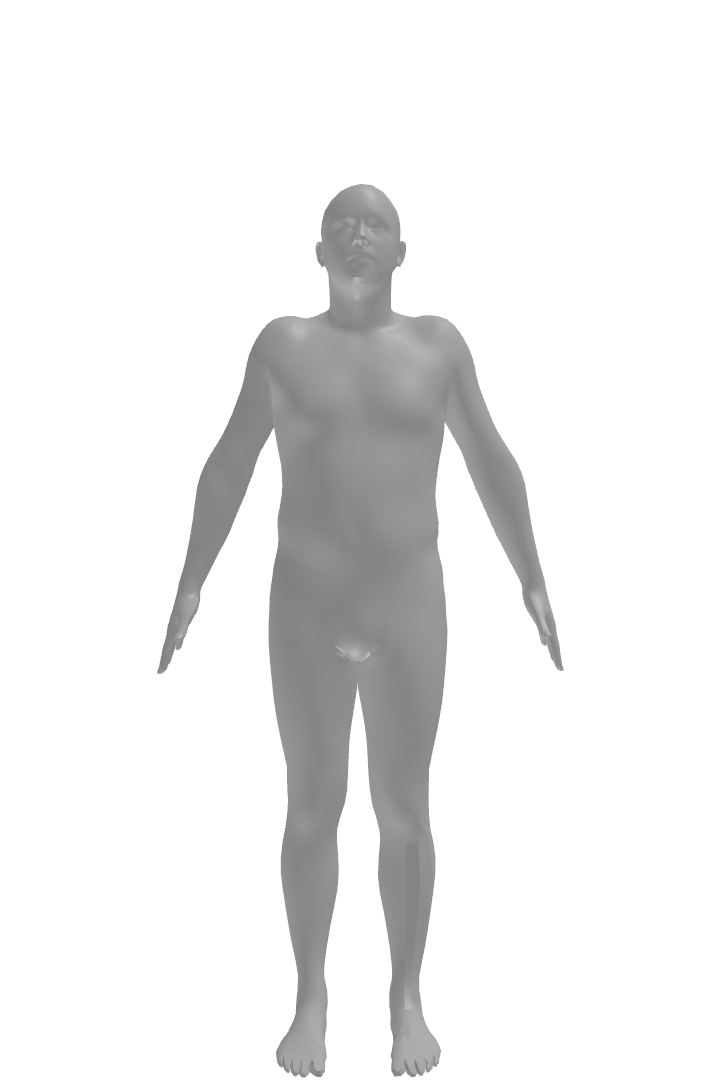
\includegraphics[width=\imgWidth]{files/visualize_betas/baseline_m}
        \includegraphics[width=\imgWidth]{files/visualize_betas/beta_0_\betaVar_m}
        \linebreak
        \includegraphics[width=\imgWidth]{files/visualize_betas/beta_0_-\betaVar_f}
        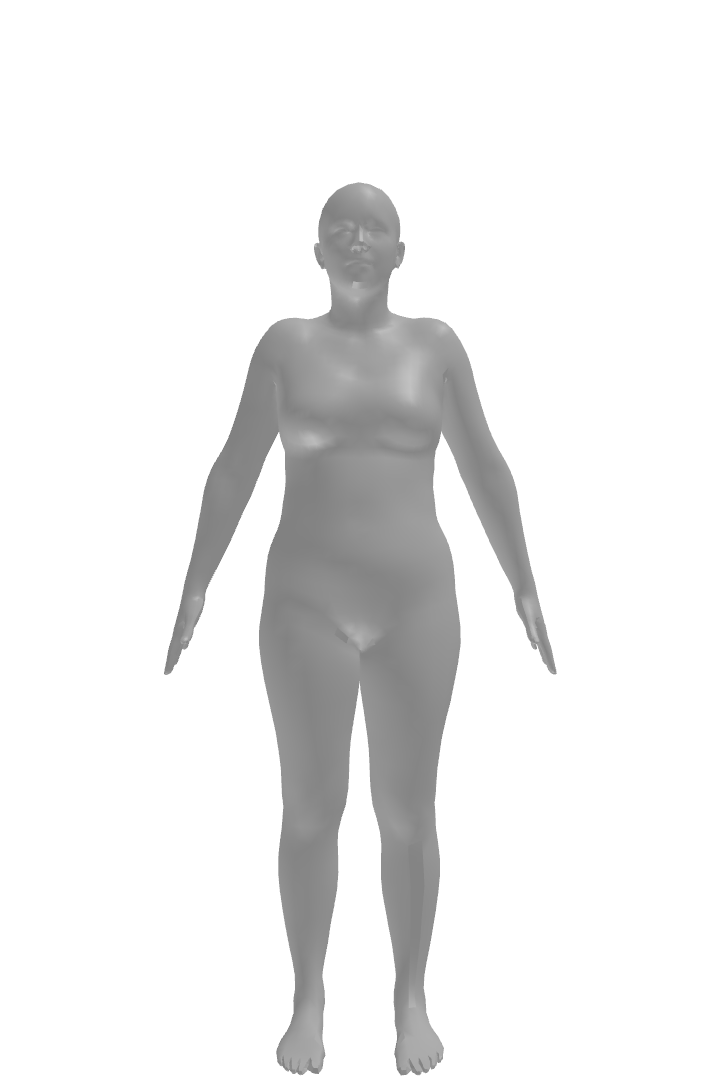
\includegraphics[width=\imgWidth]{files/visualize_betas/baseline_f}
        \includegraphics[width=\imgWidth]{files/visualize_betas/beta_0_\betaVar_f}
        \caption[Effect of varying $\beta_1$ in SMPL.]{$\beta_1 = [-\betaVar, 0, +\betaVar]$.}
        \label{fig:beta-1-vis}
    \end{minipage}
\end{figure}

\begin{figure}[ht!]
    \centering

    \begin{minipage}[b]{\textwidth}
        \centering
        \includegraphics[width=\imgWidth]{files/visualize_betas/beta_1_-\betaVar_m}
        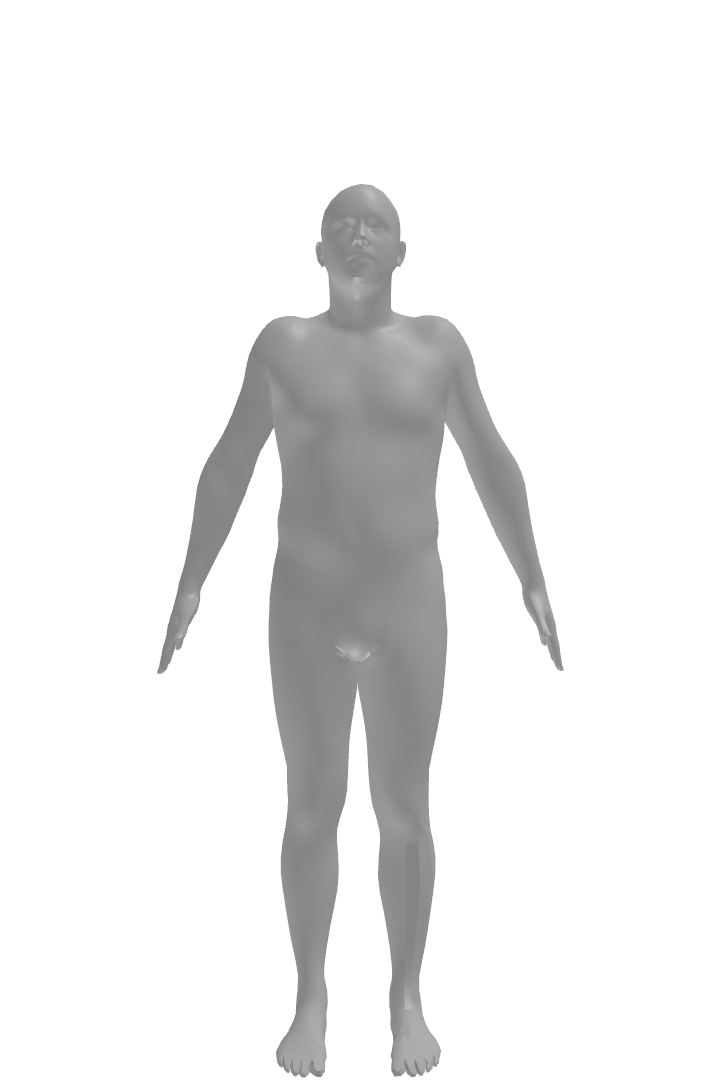
\includegraphics[width=\imgWidth]{files/visualize_betas/baseline_m}
        \includegraphics[width=\imgWidth]{files/visualize_betas/beta_1_\betaVar_m}
        \linebreak
        \includegraphics[width=\imgWidth]{files/visualize_betas/beta_1_-\betaVar_f}
        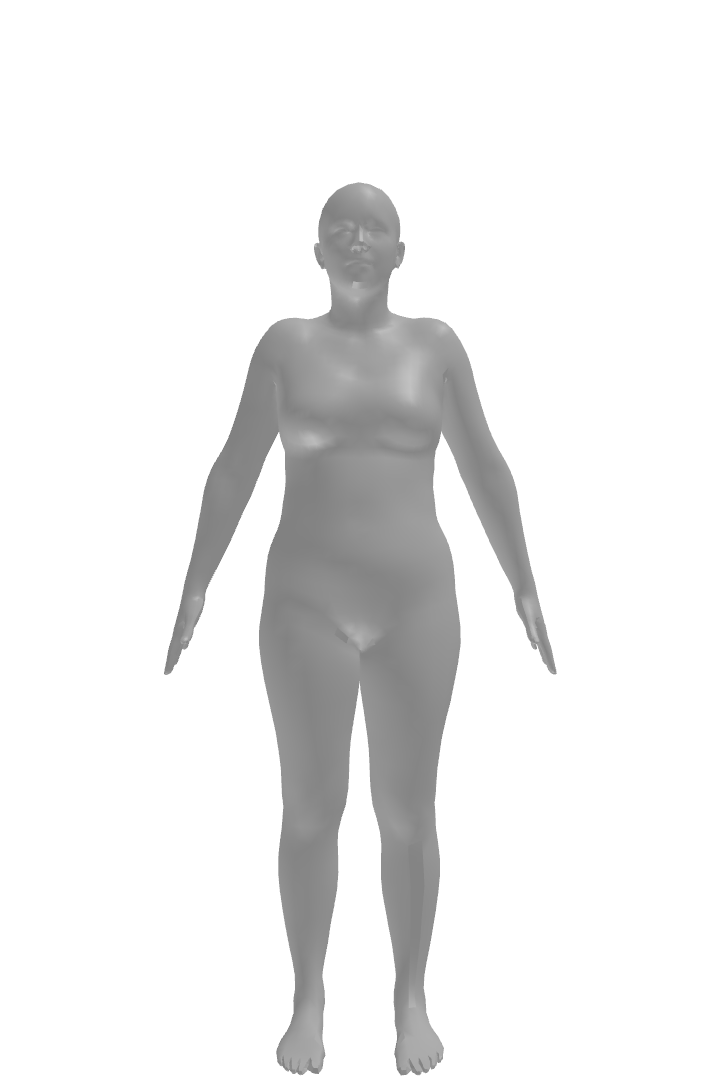
\includegraphics[width=\imgWidth]{files/visualize_betas/baseline_f}
        \includegraphics[width=\imgWidth]{files/visualize_betas/beta_1_\betaVar_f}
        \caption[Effect of varying $\beta_2$ in SMPL.]{$\beta_2 = [-\betaVar, 0, +\betaVar]$.}
    \end{minipage}
\end{figure}

\begin{figure}[ht!]
    \centering

    \begin{minipage}[b]{\textwidth}
        \centering
        \includegraphics[width=\imgWidth]{files/visualize_betas/beta_2_-\betaVar_m}
        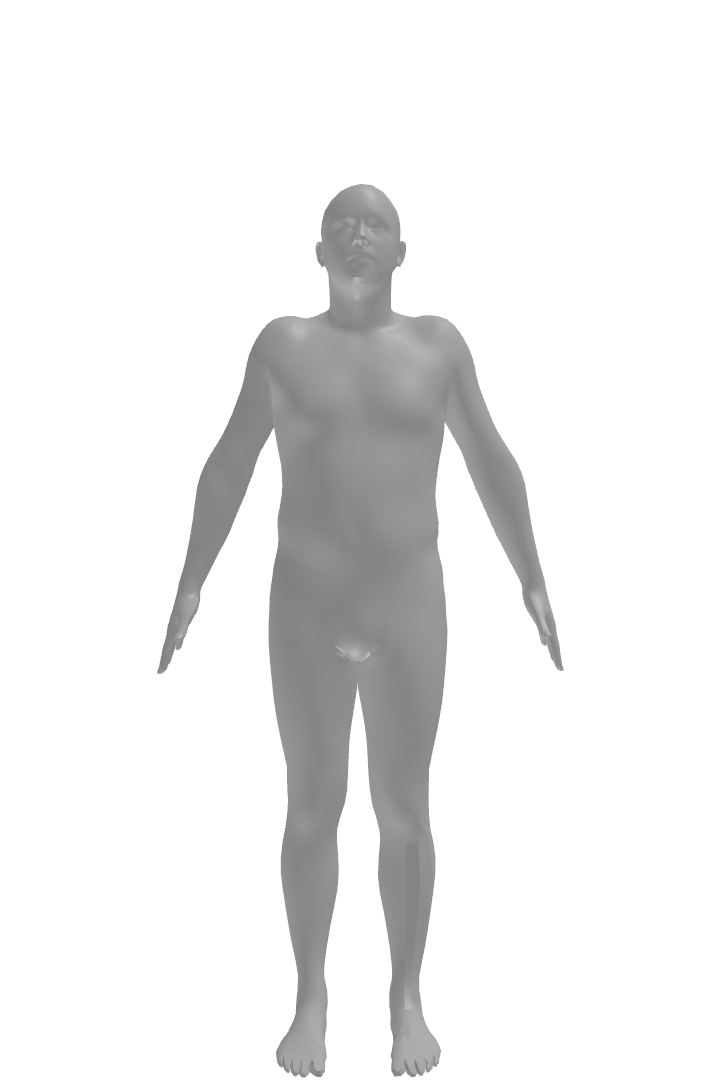
\includegraphics[width=\imgWidth]{files/visualize_betas/baseline_m}
        \includegraphics[width=\imgWidth]{files/visualize_betas/beta_2_\betaVar_m}
        \linebreak
        \includegraphics[width=\imgWidth]{files/visualize_betas/beta_2_-\betaVar_f}
        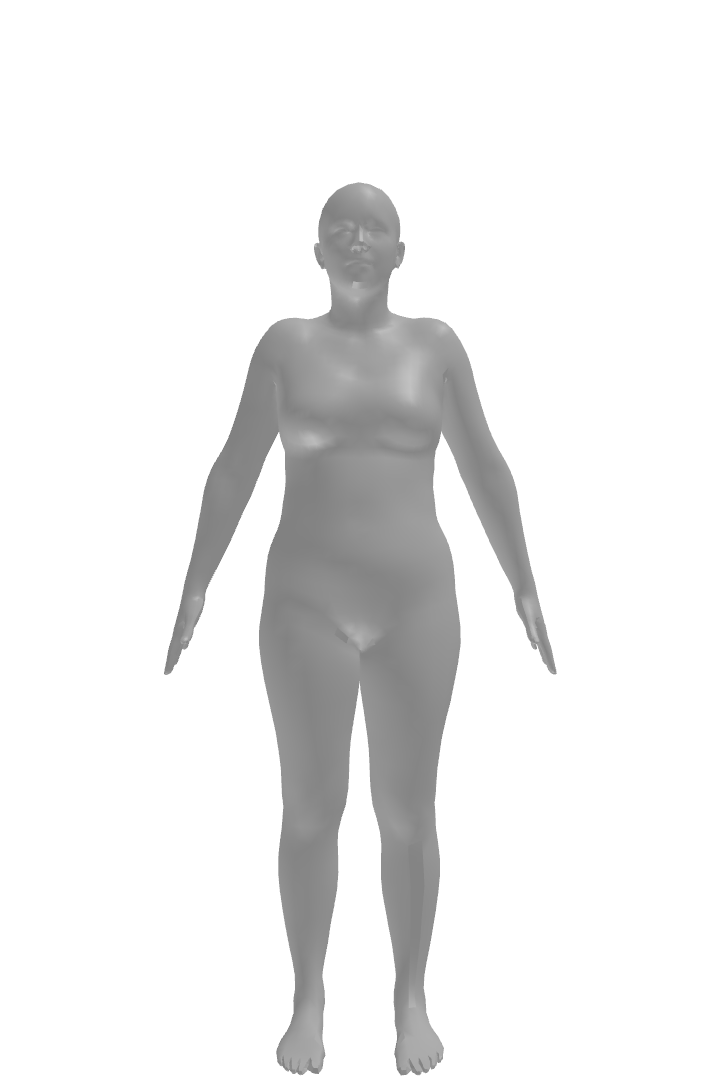
\includegraphics[width=\imgWidth]{files/visualize_betas/baseline_f}
        \includegraphics[width=\imgWidth]{files/visualize_betas/beta_2_\betaVar_f}
        \caption[Effect of varying $\beta_3$ in SMPL.]{$\beta_3 = [-\betaVar, 0, +\betaVar]$.}
    \end{minipage}
\end{figure}

\begin{figure}[ht!]
    \centering

    \begin{minipage}[b]{\textwidth}
        \centering
        \includegraphics[width=\imgWidth]{files/visualize_betas/beta_3_-\betaVar_m}
        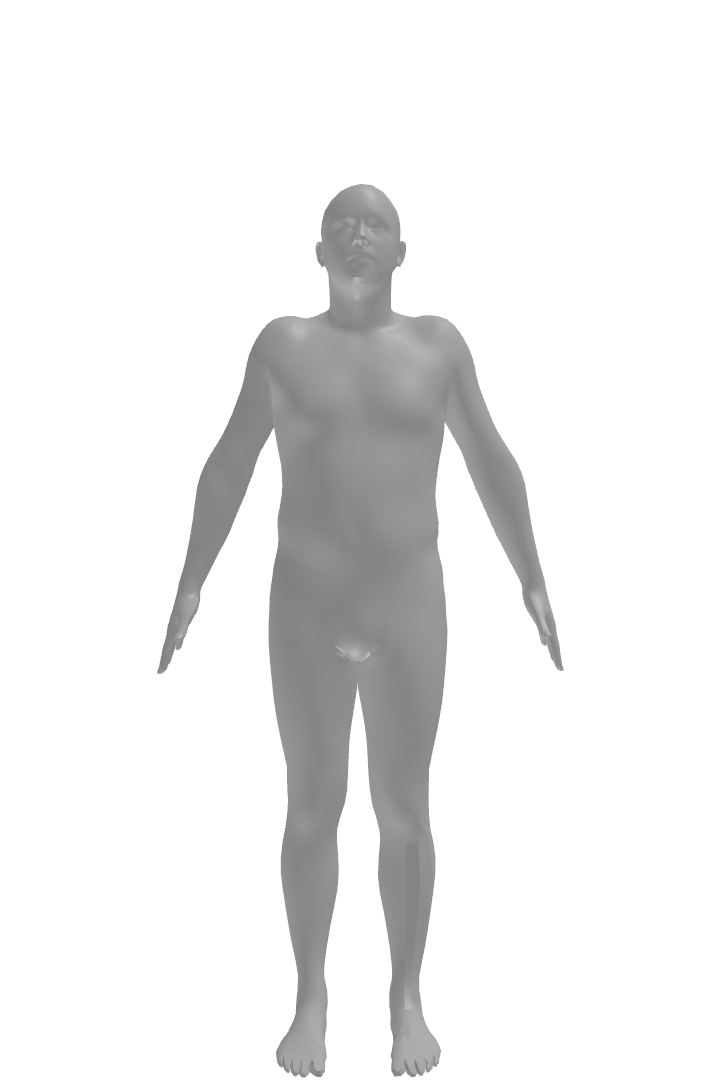
\includegraphics[width=\imgWidth]{files/visualize_betas/baseline_m}
        \includegraphics[width=\imgWidth]{files/visualize_betas/beta_3_\betaVar_m}
        \linebreak
        \includegraphics[width=\imgWidth]{files/visualize_betas/beta_3_-\betaVar_f}
        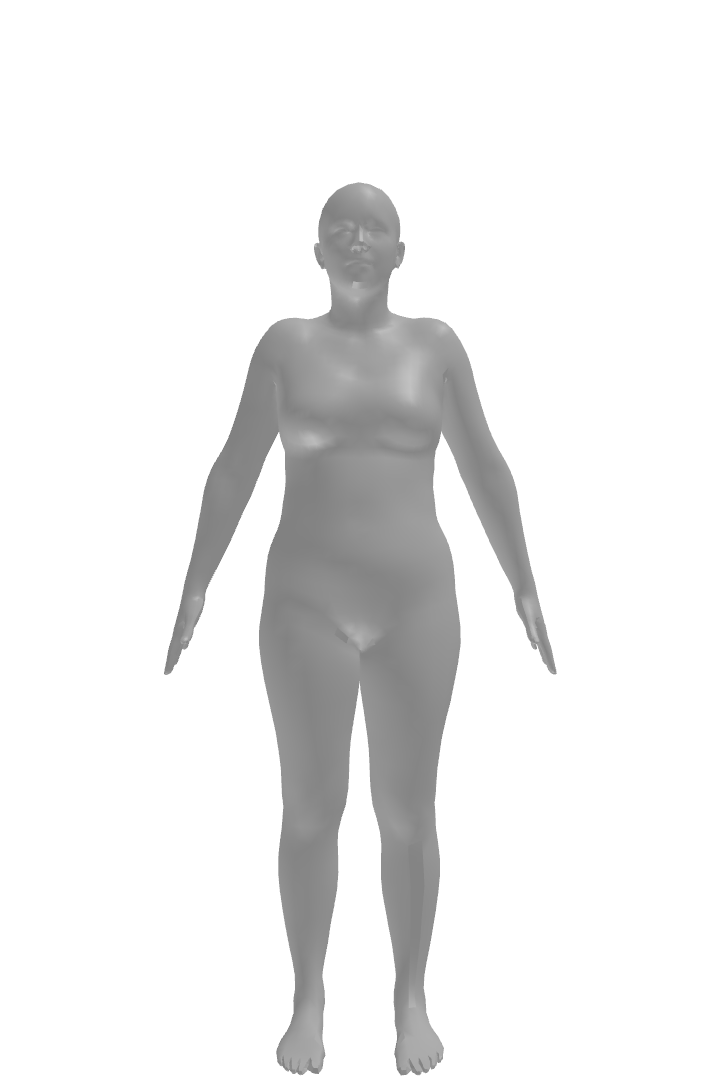
\includegraphics[width=\imgWidth]{files/visualize_betas/baseline_f}
        \includegraphics[width=\imgWidth]{files/visualize_betas/beta_3_\betaVar_f}
        \caption[Effect of varying $\beta_4$ in SMPL.]{$\beta_4 = [-\betaVar, 0, +\betaVar]$.}
    \end{minipage}
\end{figure}

\begin{figure}[ht!]
    \centering

    \begin{minipage}[b]{\textwidth}
        \centering
        \includegraphics[width=\imgWidth]{files/visualize_betas/beta_4_-\betaVar_m}
        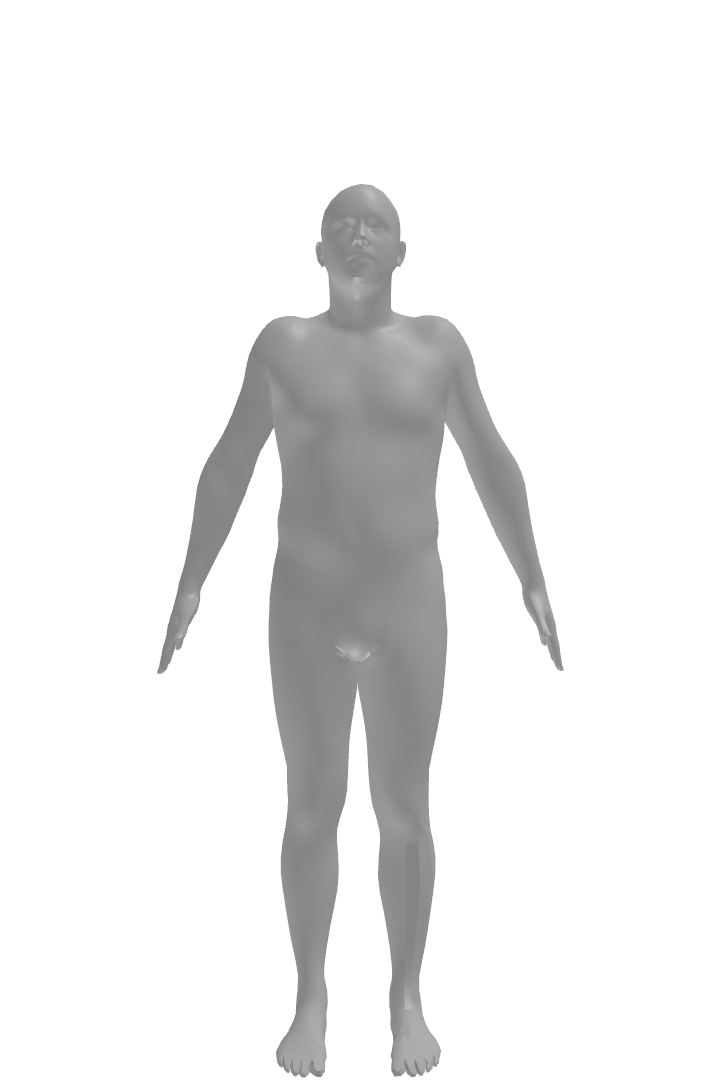
\includegraphics[width=\imgWidth]{files/visualize_betas/baseline_m}
        \includegraphics[width=\imgWidth]{files/visualize_betas/beta_4_\betaVar_m}
        \linebreak
        \includegraphics[width=\imgWidth]{files/visualize_betas/beta_4_-\betaVar_f}
        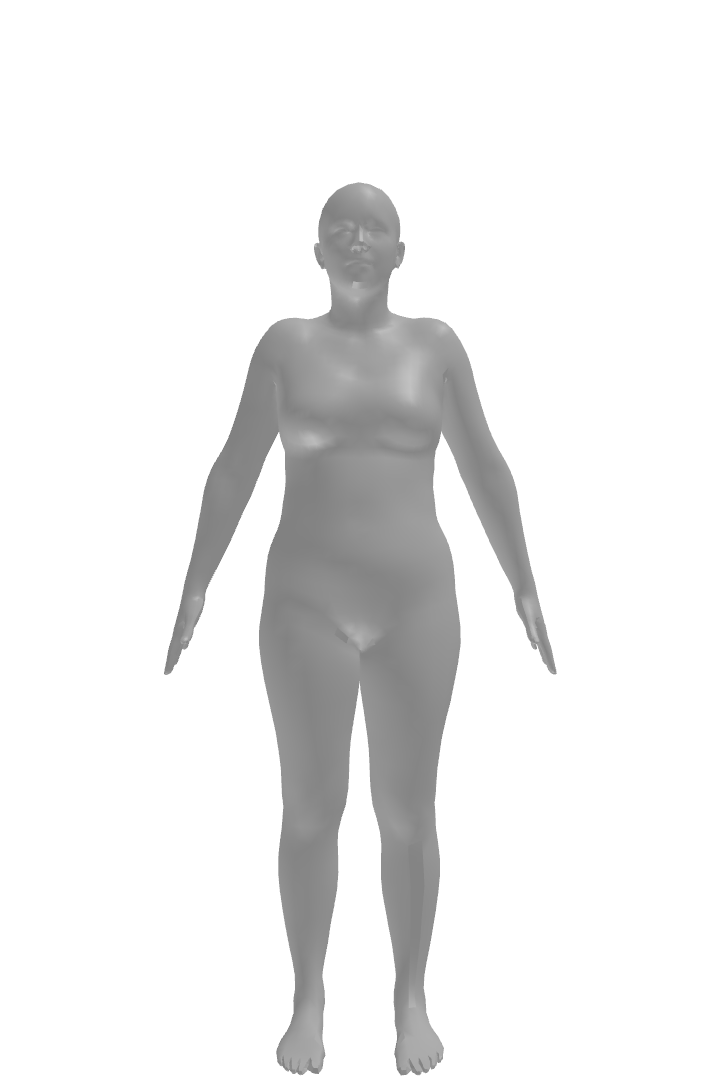
\includegraphics[width=\imgWidth]{files/visualize_betas/baseline_f}
        \includegraphics[width=\imgWidth]{files/visualize_betas/beta_4_\betaVar_f}
        \caption[Effect of varying $\beta_5$ in SMPL.]{$\beta_5 = [-\betaVar, 0, +\betaVar]$.}
    \end{minipage}
\end{figure}

\begin{figure}[ht!]
    \centering

    \begin{minipage}[b]{\textwidth}
        \centering
        \includegraphics[width=\imgWidth]{files/visualize_betas/beta_5_-\betaVar_m}
        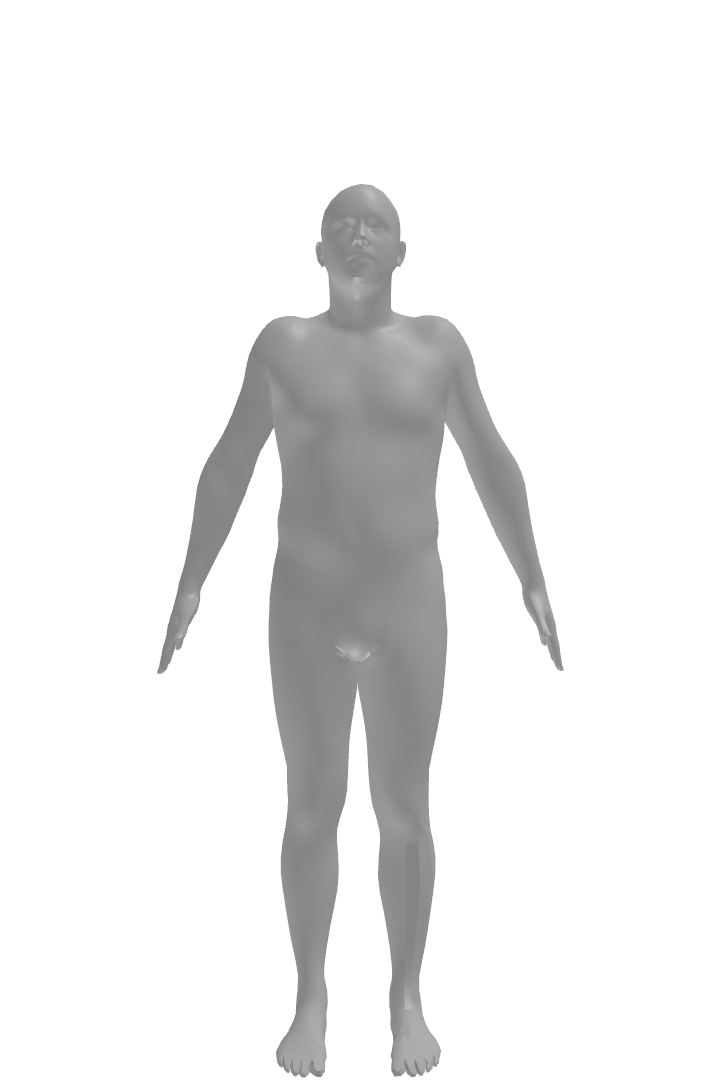
\includegraphics[width=\imgWidth]{files/visualize_betas/baseline_m}
        \includegraphics[width=\imgWidth]{files/visualize_betas/beta_5_\betaVar_m}
        \linebreak
        \includegraphics[width=\imgWidth]{files/visualize_betas/beta_5_-\betaVar_f}
        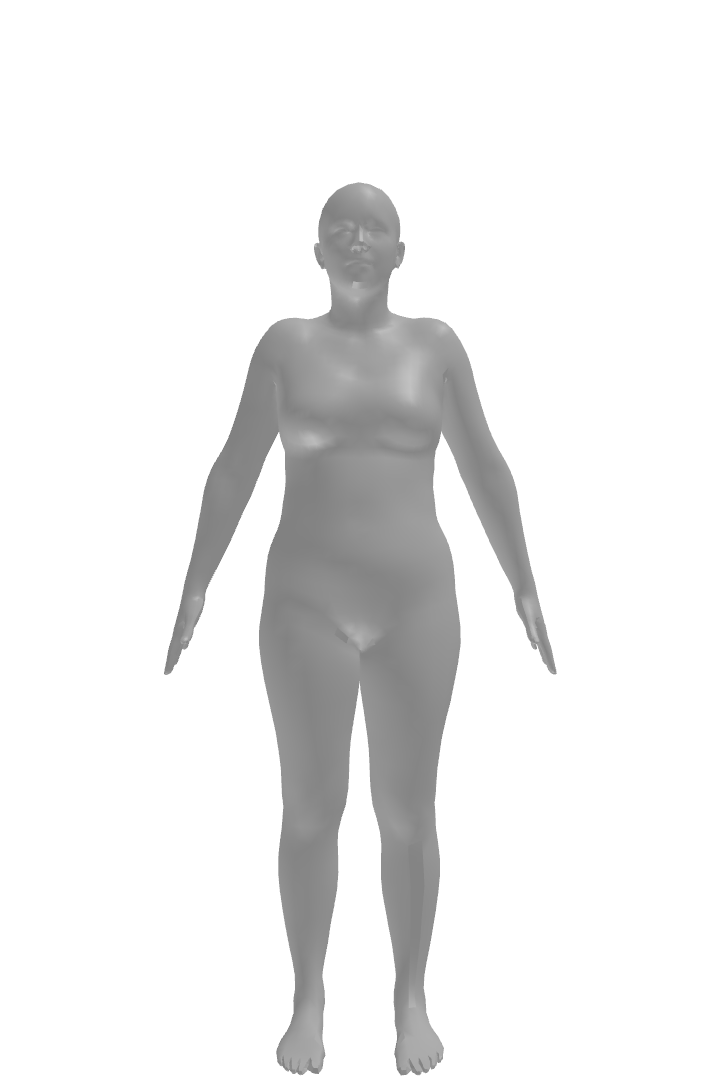
\includegraphics[width=\imgWidth]{files/visualize_betas/baseline_f}
        \includegraphics[width=\imgWidth]{files/visualize_betas/beta_5_\betaVar_f}
        \caption[Effect of varying $\beta_6$ in SMPL.]{$\beta_6 = [-\betaVar, 0, +\betaVar]$.}
    \end{minipage}
\end{figure}

\begin{figure}[ht!]
    \centering

    \begin{minipage}[b]{\textwidth}
        \centering
        \includegraphics[width=\imgWidth]{files/visualize_betas/beta_6_-\betaVar_m}
        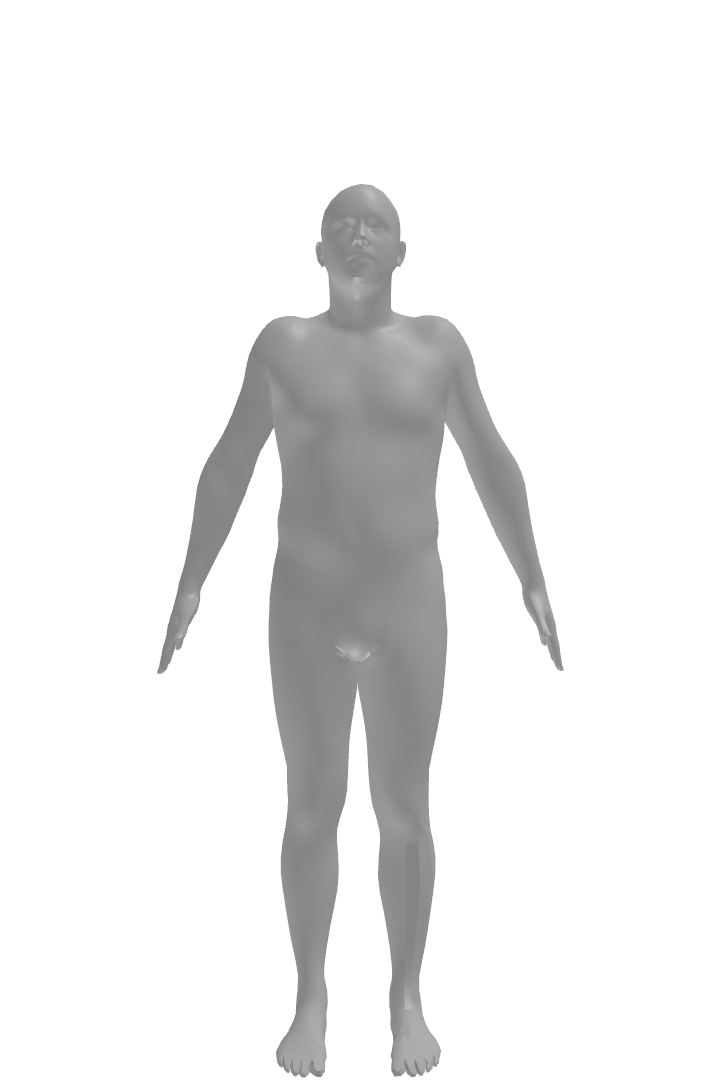
\includegraphics[width=\imgWidth]{files/visualize_betas/baseline_m}
        \includegraphics[width=\imgWidth]{files/visualize_betas/beta_6_\betaVar_m}
        \linebreak
        \includegraphics[width=\imgWidth]{files/visualize_betas/beta_6_-\betaVar_f}
        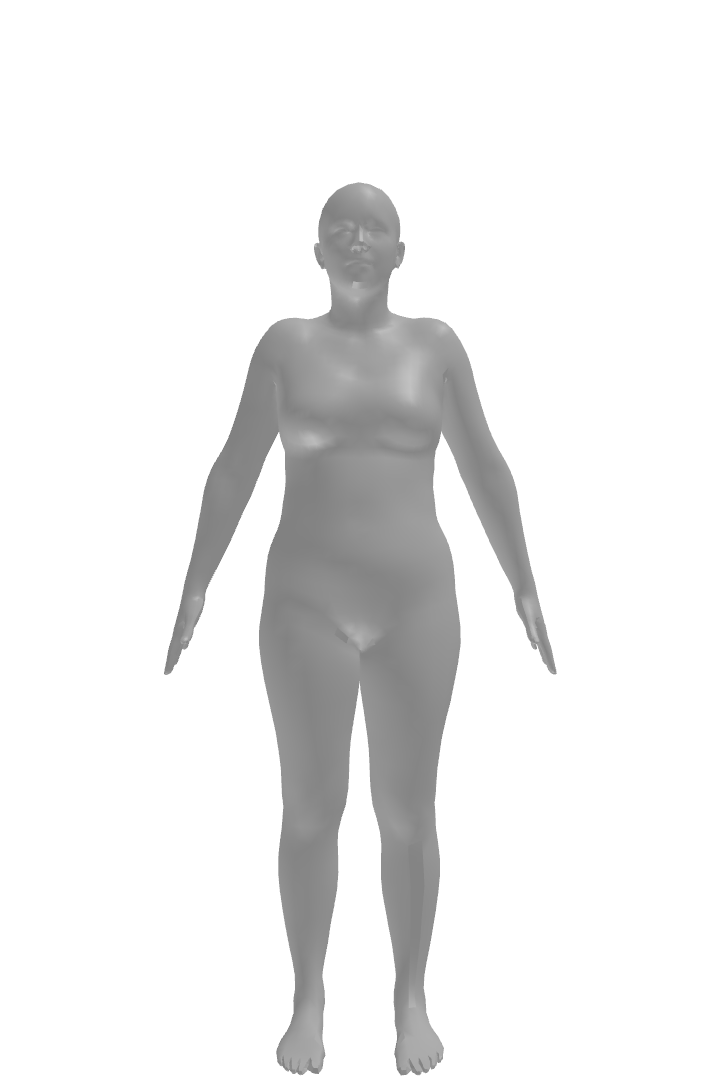
\includegraphics[width=\imgWidth]{files/visualize_betas/baseline_f}
        \includegraphics[width=\imgWidth]{files/visualize_betas/beta_6_\betaVar_f}
        \caption[Effect of varying $\beta_7$ in SMPL.]{$\beta_7 = [-\betaVar, 0, +\betaVar]$.}
    \end{minipage}
\end{figure}

\begin{figure}[ht!]
    \centering

    \begin{minipage}[b]{\textwidth}
        \centering
        \includegraphics[width=\imgWidth]{files/visualize_betas/beta_7_-\betaVar_m}
        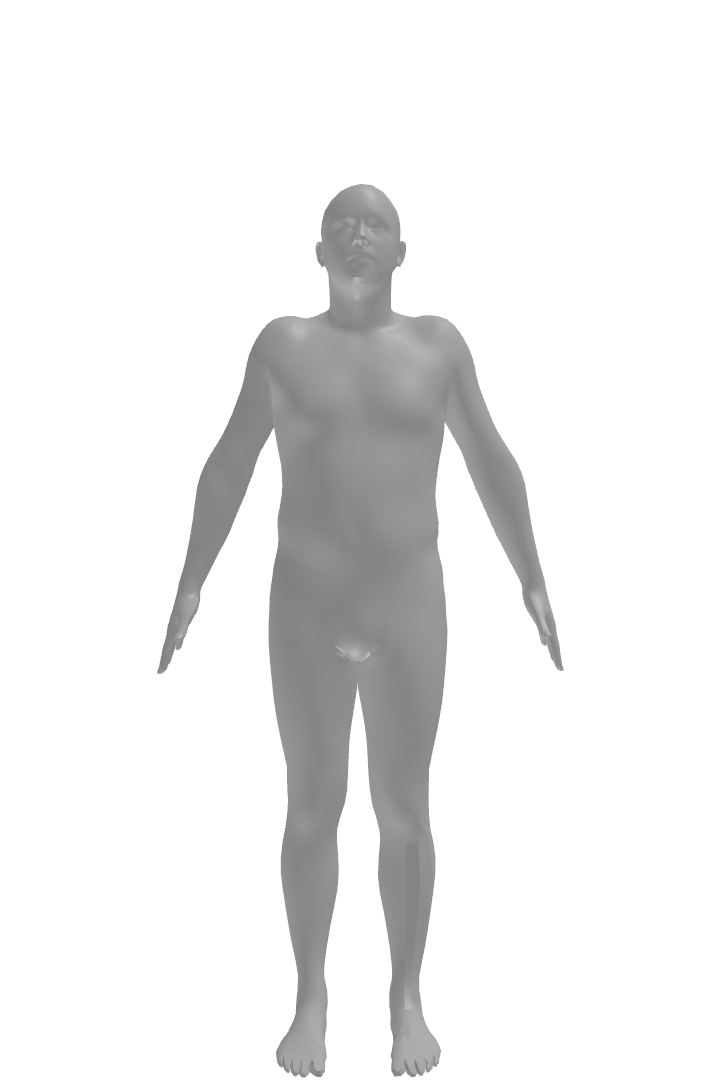
\includegraphics[width=\imgWidth]{files/visualize_betas/baseline_m}
        \includegraphics[width=\imgWidth]{files/visualize_betas/beta_7_\betaVar_m}
        \linebreak
        \includegraphics[width=\imgWidth]{files/visualize_betas/beta_7_-\betaVar_f}
        \includegraphics[width=\imgWidth]{files/visualize_betas/baseline_f}
        \includegraphics[width=\imgWidth]{files/visualize_betas/beta_7_\betaVar_f}
        \caption[Effect of varying $\beta_8$ in SMPL.]{$\beta_8 = [-\betaVar, 0, +\betaVar]$.}
    \end{minipage}
\end{figure}

\begin{figure}[ht!]
    \centering

    \begin{minipage}[b]{\textwidth}
        \centering
        \includegraphics[width=\imgWidth]{files/visualize_betas/beta_8_-\betaVar_m}
        \includegraphics[width=\imgWidth]{files/visualize_betas/baseline_m}
        \includegraphics[width=\imgWidth]{files/visualize_betas/beta_8_\betaVar_m}
        \linebreak
        \includegraphics[width=\imgWidth]{files/visualize_betas/beta_8_-\betaVar_f}
        \includegraphics[width=\imgWidth]{files/visualize_betas/baseline_f}
        \includegraphics[width=\imgWidth]{files/visualize_betas/beta_8_\betaVar_f}
        \caption[Effect of varying $\beta_9$ in SMPL.]{$\beta_9 = [-\betaVar, 0, +\betaVar]$.}
    \end{minipage}
\end{figure}

\begin{figure}[ht!]
    \centering

    \begin{minipage}[b]{\textwidth}
        \centering
        \includegraphics[width=\imgWidth]{files/visualize_betas/beta_9_-\betaVar_m}
        \includegraphics[width=\imgWidth]{files/visualize_betas/baseline_m}
        \includegraphics[width=\imgWidth]{files/visualize_betas/beta_9_\betaVar_m}
        \linebreak
        \includegraphics[width=\imgWidth]{files/visualize_betas/beta_9_-\betaVar_f}
        \includegraphics[width=\imgWidth]{files/visualize_betas/baseline_f}
        \includegraphics[width=\imgWidth]{files/visualize_betas/beta_9_\betaVar_f}
        \caption[Effect of varying $\beta_{10}$ in SMPL.]{$\beta_{10} = [-\betaVar, 0, +\betaVar]$.}
        \label{fig:beta-10-vis}
    \end{minipage}
\end{figure}


%\input{glosario/entradas_glosario}
% \addcontentsline{toc}{chapter}{Glosario} %si se usa glosario hay que añadirlo al índice
% \printglossary %muestra el glosario

\end{document}
